\documentclass[11pt]{book}

% Preamble
\usepackage{graphicx, grffile} % For including images
\usepackage{amsmath,amsfonts} % For mathematical formulas
\usepackage{hyperref} % For hyperlinks
\usepackage{geometry} % For page layout and margins
\usepackage{listings} % For code listings
\usepackage{xcolor}   % For colored text and backgrounds
\usepackage{indentfirst}   % For colored text and backgrounds

% Define code listing styles
\lstset{
    basicstyle=\ttfamily,
    keywordstyle=\color{blue},
    stringstyle=\color{red},
    commentstyle=\color{green},
    morecomment=[l][\color{magenta}]{\#}
}

% Document settings
\geometry{
    a4paper,
    total={170mm,257mm},
    left=20mm,
    top=20mm,
}

\title{\textbf{3D Visual Reconstruction: A Practical Approach}}
\author{Vahagn Yeghikyan}
\date{2023}

% Begin Document
\begin{document}

\frontmatter
\maketitle
\tableofcontents

\mainmatter

\part{Introduction to Image Processing}

\chapter{Understanding Digital Images}


\section{Introduction to Digital Imaging}

A digital image is a representation of a visual image (like a photograph or scene) in the form of a two-dimensional array composed of pixels. Each pixel, or picture element, in this array contains information about the brightness and color at a specific point in the image. Typically, each pixel represents 1 (grayscale), 3 (rgb) or 4 (rgba) values. 

%\subsection{What is a Digital Image?}
%A digital image is typically created by converting optical information (light) into electrical signals using a sensor, as found in digital cameras. This conversion process is known as digitization.

In digital imaging, a standard coordinate system is used. The origin (0,0) is located at the top-left corner of the image. The x-coordinate increases horizontally to the right, and the y-coordinate increases vertically downwards. This coordinate system is essential for accessing and manipulating pixels within an image.

\begin{figure}[h]
\centering
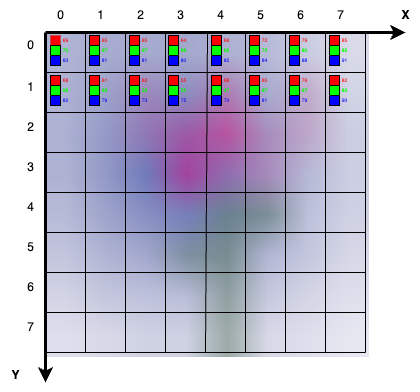
\includegraphics[width=0.6\textwidth]{images/pixels.drawio.png}
\caption{A simple 2D representation of a digital image showing its coordinate system.}
\end{figure}


Throughout this book, we will consider pixel components values encoded in 8 bits, hence, ranging from 0 (no color) to 255 (max color). There are sensors that produce higher color resolution that  are encoded into 12 and even 20 bits (expensive production photo-cameras), however, although crucial for certain applications, such a high color resolution is of no use for our purposes.   


\section{Understanding Image Formats and Compression}

Since, throughout the book we will have practical examples that use actual images, we should understand, that storing the image data as is on the hard drive is inefficient. In the world of digital imaging, different formats are used to store images, each with its unique characteristics. Some of the most common formats include BMP, JPEG, and PNG. Understanding these formats is crucial for image processing, as the choice of format can affect the quality and size of the image.

Below are 3 most common image formats that are widely used and supported.

\begin{itemize}
	\item {\bf BMP (Bitmap Image File)} The BMP format, also known as bitmap, is a simple, uncompressed format native to the Windows environment. It stores color data for each pixel in the image without any compression. As a result, BMP files are typically large but maintain high image quality.
	\item {\bf JPEG (Joint Photographic Experts Group)} JPEG is a widely used format for photographic images. It employs lossy compression, which reduces file size by selectively discarding less important data. While this compression can significantly reduce file sizes, it can also lead to a loss of image quality, especially at higher compression levels.
	\item {\bf PNG (Portable Network Graphics)} PNG is a format designed for the web, offering lossless compression. It provides a good balance between image quality and file size and supports transparency, making it suitable for graphics and web images.
\end{itemize}


While understanding image formats and compression is vital, the implementation details of these compression algorithms are beyond the scope of this book. Our focus will primarily be on the processing and manipulation of images, regardless of their format. However, knowledge of these formats is essential when choosing the right format for storage and processing tasks in image processing and 3D reconstruction applications.


\section{Practical Application: The Image Class}


Moving from the theoretical understanding of digital images, let's delve into a practical implementation. This will enable us to understand the digital images better by playing with the actual data. In our accompanying library, we have an `Image` class, defined in `image.h`, which encapsulates the properties and functionalities of a digital image in C++. 

The `Image` class serves as a fundamental building block in our library. It holds the image data and provides methods to access and manipulate pixels. The class is designed to be flexible and efficient, suitable for a range of image processing tasks.

Here is the code listing for the `Image` class:

\begin{lstlisting}[language=C++, caption={Image class implementation}]
#ifndef VISQ_IMAGE_H
#define VISQ_IMAGE_H

#include <memory> // for shared_ptr

namespace visq {

template<typename T>
class Image {
 public:
  Image(size_t width, size_t height, size_t channels)
    : width_(width), height_(height), channels_(channels),
      stride_(width * channels), offset_(0),
      data_(new uint8_t[width * height * channels]) {}

  Image(const Image<T>& other, size_t new_width, size_t new_height, size_t offset)
    : width_(new_width), height_(new_height), channels_(other.channels_),
      stride_(other.stride_), offset_(offset),
      data_(other.data_) {}

  void Set(T value, size_t y, size_t x, size_t c) {
    data_.get()[(y * stride_) + (x * channels_) + c + offset_] = value;
  }

  [[nodiscard]] const T& At(size_t y, size_t x, size_t c) const  {
    return data_.get()[(y * stride_) + (x * channels_) + c + offset_];
  }

  T* Data() {
    return data_.get();
  }

  [[nodiscard]] const T* Data() const {
    return data_.get();
  }

  template<typename R>
  bool CopyTo(Image<R> &other) const;

  [[nodiscard]] bool IsContinuous() const {
    return stride_ == width_ * channels_;
  }

  // Getters
  [[nodiscard]] size_t GetWidth() const { return width_; }
  [[nodiscard]] size_t GetHeight() const { return height_; }
  [[nodiscard]] size_t GetChannels() const { return channels_; }
  [[nodiscard]] size_t GetStride() const { return stride_; }
  [[nodiscard]] size_t GetOffset() const { return offset_; }

 private:
  size_t width_;
  size_t height_;
  size_t channels_;
  size_t stride_;
  size_t offset_;
  std::shared_ptr<T[]> data_;
};

}  // namespace visq

#endif  // VISQ_IMAGE_H
\end{lstlisting}

Let us quickly review the basic properties of the class.

\begin{itemize}
	\item {\bf width\_} The width of the image in pixels.
	\item {\bf height\_} The height of the image in pixels.
	\item {\bf channels\_} The number of channels (typically 1, 3, or 4).
	\item {\bf data\_} A shared pointer to the pixel data itself. We will keep the pixel data in the most common - interleaved format, i.e. the first $channels\_$ bytes will represent the top left pixel components, the next $channels\_$ bytes the pixel to the right and so on until we reach the end of the top row. Then comes the second row with the exact same format.   
\end{itemize} 

We will speak about the $stride\_$ and $offset\_$ variables a bit later. For now, we will think about the simplest case where $offset\_ = 0$ and $stride\_ = width\_ * channels\_$.   

- \textbf{Pixel Access}: The `At` method provides direct access to the pixel values, enabling both read and write operations. An implementation of such a method can look as follows:

 \begin{lstlisting}[language=C++, caption={An implementation of the method At}]
 uint8_t & Image::At(size_t y, size_t x, size_t channel) {
   return data_[y_ * width_ * channels_ + x_* channels_ + channel];
 }	
 \end{lstlisting}

Here and there we would want, however, to access not the entire image, but a small part of it represented by a rectangle with its top-left corner located at some point $(left\_x, top\_y)$ and which has some $width$ and $height$. This is why we need the second constructor. For multiple purposes, we do not want to copy the pixel data, so we will just take the pointer to it. This, however, leads to the problem that the current implementation of the method $At$ will not work for such sub-images. Indeed $y* width\_ * channels\_$ no more represents the offset of the row. We need to now the width of the initial image and that is what we will keep in our stride variable. We will also need the $offset\_$ variable that represents the offset of the top-left pixel of the sub-image in the data array. Hence, the modified method will read:

 \begin{lstlisting}[language=C++, caption={An implementation of the method At}]
 uint8_t & Image::At(size_t y, size_t x, size_t channel) {
   return data_[offset_ + y_ * stride_ + x_* channels_ + channel];
 }	
 \end{lstlisting}


This class forms the foundation for more advanced image processing and 3D reconstruction techniques that will be explored later in the book.


As soon as we have our `Image` class we would want to load an actual image and explore its contents. However, as already mentioned, images are stored and distributed in special formats. For the implementation of image loading and saving, we utilize the `stb` library, a popular set of single-file public domain libraries for C/C++. The `stb` library provides simple and efficient solutions for handling common operations in image processing, such as reading and writing different image file formats.

\textit{Note:} The `stb` library is external to our library and must be included separately. It offers functions like `stbi\_load` and `stbi\_write\_xxx` for dealing with various image formats.


The `io.h` file in our library interfaces with the `stb` library functions and provides a simplified and unified API for our image processing tasks. It abstracts the complexities involved in directly using the `stb` library functions, thereby making image I/O operations more accessible and straightforward for users.


Now, we are ready to implement our first application. The following program will load an image and print the values of the provided channel:

\begin{lstlisting}[language=C++, caption={A simple application that prints some pixel values}]
#include <iostream>
#include "image.h"
#include "io.h"

int main(int argc, char *argv[]){

  char * imname = argv[1];
  size_t channel, print_square_size;
  char * error;
  channel = strtol(argv[2], &error);
  
  if(error){
    std::cout << error << std::endl;
    return 1;
  }
  
  print_square_size = strtol(argv[3], &error);
  if(error){
    std::cout << error << std::endl;
    return 1;
  }
  
  auto [error_code, Image] = LoadImage(im_path);
  if(error_code != OK)
    return 1;
  
  // some checks here.
  
  for(size_t y = 0; y < print_square_size; ++y){
    for( size_t x = 0; x < print_square_size; ++x){
      std::cout << image.At(y,x,channel) << '\t';
    }
    std::cout << std::endl;
  }
  
  return 0
}	
 \end{lstlisting}

\newpage
\section{Images as Signals}

Signal processing is a field that deals with the analysis, modification, and synthesis of signals. A signal, in a broad sense, is a function conveying information about the behavior or attributes of some phenomenon. In most cases signals are continuous smooth functions of time. Take, for example, the sound wave emitted by a source(say, speaker) or the distance of the car from its initial point through a trip.  

In the digital world, however, we cannot possibly keep the whole signal because it will potentially require memorizing an infinite  (continuum or even countable) set of pairs (t, f). Typically, in the digital world we take discrete values and store them with a certain precision (8-64bit float/integer). This process is called "sampling". Figure \ref{fig:signal} shows an example of a real world signal (the solid graph line) and the sampled digital values (black circles). 

It is clear, that during the sampling process we lose a huge amount of information. ( In fact, in some hard-core mathematical we lose almost all the information).  Should we try to recover the original signal, we will figure out that it can be done in infinitely many ways. Indeed, there are infinitely many ways to connect 2 dots with continuous functions. 

In the context of digital systems, signals are typically represented in discrete form. 
\begin{figure}[h]
\centering
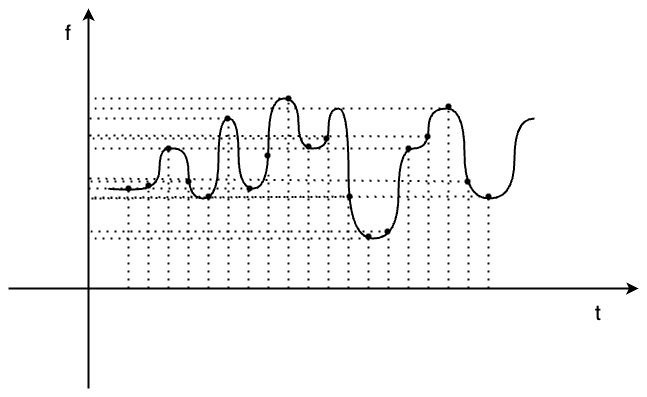
\includegraphics[width=0.6\textwidth]{images/digitalization.drawio.png}
\caption{Example of signal with its discretization}
\label{fig:signal}
\end{figure}

\begin{figure}[h]
\centering
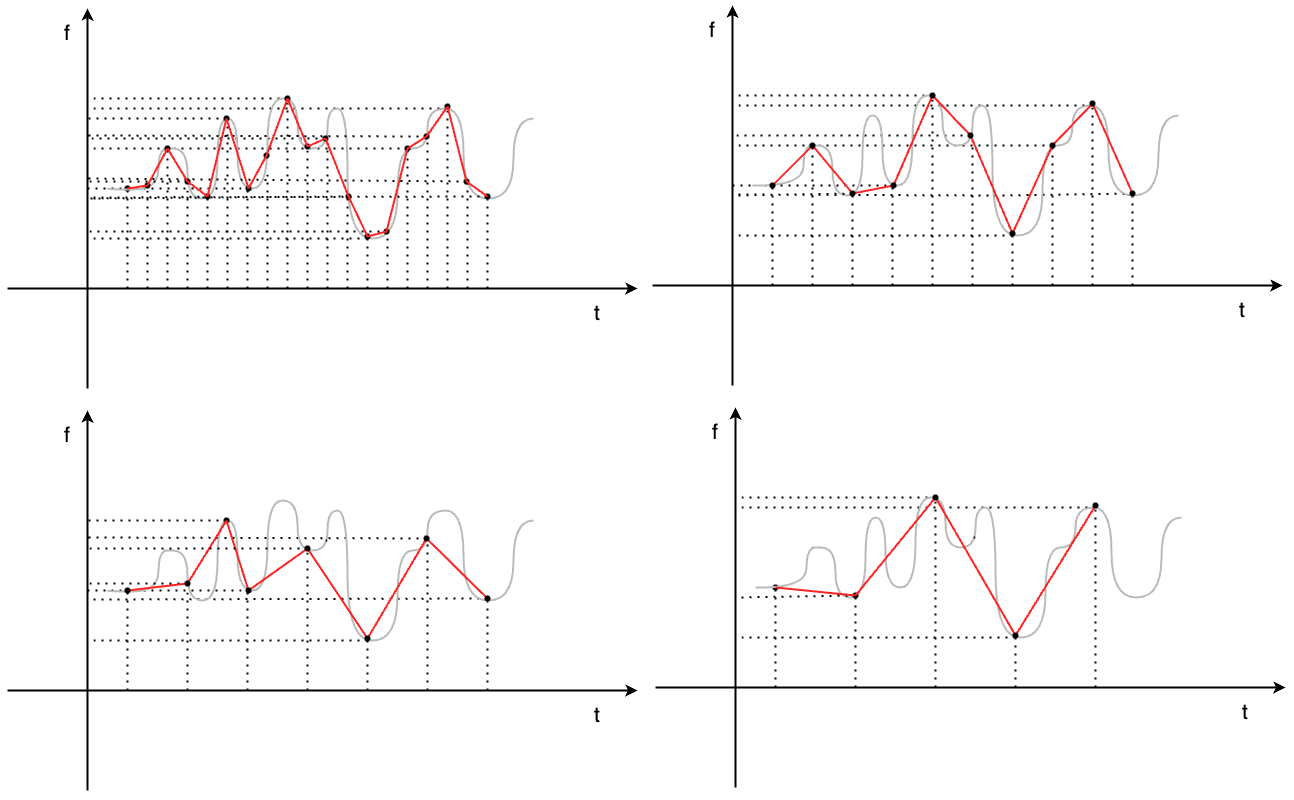
\includegraphics[width=0.6\textwidth]{images/restore-combined.png}
\caption{Example of signal with its discretization}
\label{fig:signal}
\end{figure}

 
As you see, although the figure composed of the black circles resembles the original signal, the details between the dots are omitted and lost. Restoring the values at any real time-point $t$ can be done in infinitely many ways, and, strictly speaking is not a well-defined problem.

In many applications, however, this does not matter much. The most common example of this is the sound. A typical human ear can hear sounds with frequencies in range 20Hz-20kHz. So,  


Signal processing techniques are fundamental in various scientific and engineering domains, including communications, audio processing, and image analysis.

Traditionally, signals are thought of as 1D functions, such as audio signals, which vary over time. However, images can be conceptualized as 2D signals. In this perspective, an image is a function that varies over two spatial dimensions, representing the intensity or color of light at each point.

This conceptualization allows us to apply signal processing techniques to image analysis. For instance, filtering, which is widely used in audio processing, can be applied to images for enhancement, noise reduction, or feature extraction. In this prospect we can think about the image as a 2D function $Im(y,x)$. Here and further in this section we will neglect the channels and consider only monochromatic images. 

\subsection{Resampling of Digital Signals}

One of the most common signal processing techniques is the so-called resampling. It involves changing the sampling rate or dimensionality of a signal. 

Consider a 1D signal, such as an audio waveform. Resampling might involve increasing the sampling rate (interpolation) to make the signal smoother or decreasing it (decimation) to reduce the size of the data. In both cases, we should assume that the discrete data we have, is some digitalization of a continuous signal and we should "guess" the values of the original signal in between the value with integer coordinates. We will see many examples of resampling below. A first and the most obvious example is image resize.



\subsection{Image resize}

Suppose, we want to transform an image of size $M\times N$ to the new size $M'\times N'$. The point with integer coordinates $(x',y')$ on the resized image naturally corresponds to the point 
\begin{equation}
	x = \frac{M}{M'} x',\quad y=\frac{N}{N'}y'
\end{equation} 
of the original image. Notice, that $x$ and $y$ are not necessarily integers. We know the values of the pixels in the original image only at integer coordinates. In order to guess the value at point with arbitrary real coordinates, we should interpolate the value of the continuous function $Im(x,y)$ based on the integer sampling.
 
The image Fig \ref{fig:resize} image illustrates resizing a $6\times 6$ image to $5\times 5$ pixels. The point with coordinates (1,1) corresponds to the point (1.2,1.2) in the original image. 


\begin{figure}[h]
\centering
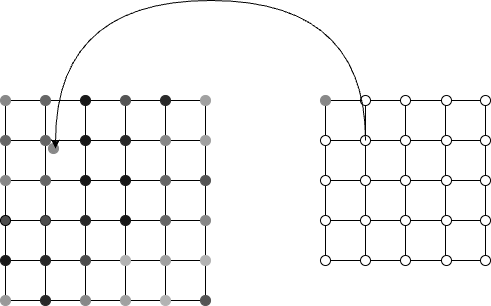
\includegraphics[width=0.6\textwidth]{images/resampling.drawio.png}
\caption{A simple 2D representation of a digital image showing its coordinate systvem.}
\label{fig:resize}
\end{figure}

There are various techniques for interpolating the value of the original image at non-integer points. Below we will describe some of them separately. The follwoing is an abstract interface that represents an interpolated image:


\begin{lstlisting}[language=C++, caption={The interface for image sampler}]
namespace visq {

/*!
 * Interface that represents an image sampler.
 */
template<typename T>
class Sampler {
public:
  Sampler(const Image<T> & image): image_(image) {};
  virtual ~Sampler() = default;

  /*!
   * Returns the interpolated value of provided image volume at real point (x,y, channel)
   */
  [[nodiscard]] virtual T Interpolate(double y, 
                                      double x,
                                      size_t channel) const = 0;

protected:
  const Image<T> image_;
};

}
\end{lstlisting}


Having defined this interface we can easily implement a generic resize logic as follows:

\begin{lstlisting}[language=C++, caption={The implementation of resizer using sampler}]
#include <visq/image.h>
#include <visq/transform/sampler.h>

namespace visq {
/*!
 * @brief Resizes image from Sampler
 */
template<typename T>
class Resizer {
public:
  /*!
   * @brief Resizes the image into the provided one.
   * @param sampler The sampler of original image.
   * @param image_to The target image to resize image to.
   */
  static void Resize(const Sampler<T> * const sampler, Image<T> * image_to) {
    double scale_x = static_cast<double>(sampler->GetImage().GetWidth()) /  image_to->GetWidth();
    double scale_y = static_cast<double>(sampler->GetImage().GetHeight()) /  image_to->GetHeight();
    for(size_t y = 0; y < image_to->GetHeight(); ++y) {
      double y_o = scale_y * y;
      for(size_t x = 0; x < image_to->GetWidth(); ++x) {
      double x_o = scale_x * x;
        for(size_t c = 0; c < image_to->GetChannels(); ++c) {
          image_to->Set(sampler->Interpolate(y_o, x_o, c), y,x,c);
        }
      }
    }
  }
};
} // namespace visq
\end{lstlisting}

\subsubsection{Nearest-neighbor interpolation}

This is the simplest and roughest interpolation. It simply returns the value of the pixel that is nearest to the point of interest. 

The following is a self-explanatory implementation:

\begin{lstlisting}[language=C++, caption={An implementation of the Nearest Neighbor interpolation}]
#include <visq/transform/sampler.h>

namespace visq {

template<typename T>
class NearestNeighborInterpolation: public Sampler<T> {
public:
  NearestNeighborInterpolation(const Image<T> & image): Sampler<T>(image) {}

  [[nodiscard]] uint8_t Interpolate(double y, double x, size_t channel) const override {
    y = std::max(0., y);
    y = std::min(static_cast<double>(this->image_.GetHeight()), y);

    x = std::max(0., x);
    x = std::min(static_cast<double>(this->image_.GetWidth()), x);

    size_t y_int = std::round(y);
    size_t x_int = std::round(x);

    return this->image_.At(y_int, x_int, channel);
  }
};

}
\end{lstlisting}

\subsubsection{Bi-linear interpolation} 

The idea behind this kind of interpolation is as old as the calculus itself. Assuming we have sampled a data from a 1-dimensional signal and got some number $N$ of data-points ($x_n, y_n)$. As the most simplistic interpolation we can simply connect the data points on the graph with lines thus filling the gaps between them.

 Namely,  we interpolate the original data with a set of linear functions as follows:

\begin{equation}
y(x) = \left\{y_k + \frac{y_{k+1} - y_{k}}{x_{k+1} - x_k} (x - x_k), \quad x_k \leq x \leq x_{k+1}\right.
\end{equation}

 Fig.\ref{fig:linear_interpolation} illustrates this.
 
\begin{figure}[h]
\centering
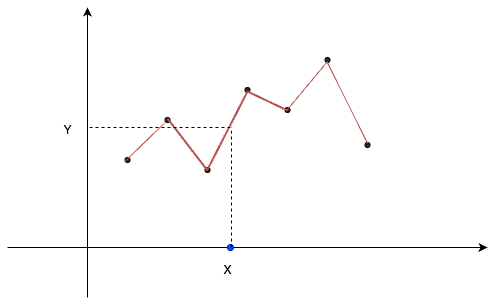
\includegraphics[width=0.6\textwidth]{images/lin.drawio.png}
\caption{Linear interpolation}
\label{fig:linear_interpolation}
\end{figure}

The bilinear interpolation is done in 2 steps, see Fig \ref{fig:bilinear_interpolation}. First The values of the points $E$ and $F$ are interpolated from the points $A,B$ and $C,D$ respectively. Then the value of the point is interpolated from the point $E$ and $F$. 

\begin{figure}[h]
\centering
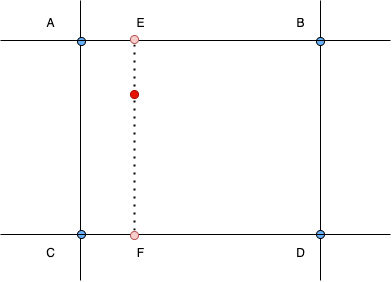
\includegraphics[width=0.6\textwidth]{images/bilin.drawio.png}
\caption{Bilinear interpolation}
\label{fig:bilinear_interpolation}
\end{figure}

It is an exercise to check that the result of interpolation does not depend on the order of interpolation, i.e. we could have performed the same steps by interpolating points on the vertical axis from point $A,C$ and $B,D$ respectively and then perform the second interpolation between those points. 


\subsubsection{Bi-Cubic Interpolation}
Cubic interpolation uses the values of neighboring points to compute a cubic polynomial for each interval between known points. In images, bicubic interpolation, which applies cubic interpolation in both dimensions, provides smoother results than linear interpolation but at a higher computational cost.
...

\subsubsection{Higher-Order Interpolation}
More sophisticated interpolation methods, such as spline interpolation or Lanczos resampling, use higher-order polynomials or specially designed kernels. These methods can provide superior results, especially for high-resolution images, but are computationally more intensive.



\subsubsection{Choosing the Right Interpolation Method}
The choice of interpolation method depends on various factors, including:
\begin{itemize}
    \item The nature of the data or image being processed.
    \item The desired balance between image quality and computational efficiency.
    \item The specific requirements of the application, such as real-time processing constraints or the need for high-quality visual results.
\end{itemize}

Each method has its advantages and trade-offs. Nearest-neighbor interpolation, while less computationally demanding, may not be suitable for high-quality image scaling. On the other hand, methods like bicubic interpolation or Lanczos resampling, while offering higher quality, might be overkill for simple applications or when computational resources are limited.

In the following sections, we will explore these interpolation methods in more detail, particularly in the context of image processing tasks such as resizing and geometric transformations.

% Add more chapters and parts as needed	

\section{Fourier transform}

It is impossible to underestimate the importance of Fourier transform in signal processing. Here we assume that the reader is familiar with the theory from a basic course of calculus and hence, to keep the context we are going just to copy the definitions here and highlight properties that are important for our purposes.

\subsection{Finite case}

Let us have a function $f(t)$ defined on an interval $ 0 \leq t \leq T$. Then, given the function satisfy certain conditions (which are presumed) it can be represented as an infinite sum of harmonic functions:

\begin{equation}
f(t) = \sum\limits_{n=0}^\infty \left(A_n \cos{\omega_n t} + B_n \sin{\omega_n t}\right), \text{ where } \omega_n = \frac{2 \pi n}{T}\label{fourier_finite}
\end{equation}

The coefficients $A_n$ and $B_n$ can be computed from the initial function as follows:

\begin{equation}
A_n = \frac{2}{T}\int\limits_{t=0}^T f(t) \cos{\omega_n t} dt,\quad B_n = \frac{2}{T}\int\limits_{t=0}^T f(t) \sin{\omega_n t} dt\label{fourier_finite_coefficients}
\end{equation}

Given these integrals exist, the proof follows from the simple properties of harmonic functions

\begin{equation}
\int\limits_{t=0}^T \cos{\omega_n}y \cos{\omega_kt} dt = \int\limits_{t=0}^T \sin{\omega_n}y \sin{\omega_kt} dt = \frac{T}{2}\delta_{nk},\quad \int\limits_{t=0}^T \cos{\omega_n}y \sin{\omega_kt} dt = 0
\end{equation}

The formula \eqref{fourier_finite} can be interpreted as any finite smooth function $f(t)$ can be represented as a superposition of monochromatic waves with certain amplitude and phase. This fact as we will see later is of crucial importance in the study of the properties of a signal. Indeed, since both expressions \eqref{fourier_finite} and \eqref{fourier_finite_coefficients} are linear by $f(t)$ allows us in many cases to investigate the changes of well known harmonic functions and then assemble back to the to the otherwise complex function $f$.

The formula \eqref{fourier_finite} can be written in complex form:

\begin{equation}
f(t) = \sum\limits_{n=0}^\infty C_n e^{\imath \omega_n t},\label{fourier_finite_complex}
\end{equation}

where complex coefficients $C_n$ play the role of complex amplitudes:

\begin{equation}
C_n = \frac{1}{T} \int\limits_{0}^T f(t) e^{-\imath \omega_n t}dt
\end{equation}

\subsection{Discrete case}


In the digital world the signals cannot be stored continuously. In other words, of all continuum set of pairs $(t, f)$ we reduce to a finite set of pairs $(t_n, f_n)$. The price is that we lose a lot of information about the initial signal. We would like to be able to extend formulae  \eqref{fourier_finite} and \eqref{fourier_finite_coefficients} for this case. Before we obtain a correct modification, let us observe some peculiar effect that comes from sampling.

\subsubsection{Aliasing}

Let us consider a harmonic signal on interval $[0,T]$ sampled with $N$ values separated with $N-1$ intervals with length $T/N$ each. Among all possible frequencies we are interested in one of those from \eqref{fourier_finite}. In the most general case the signal has the following form:

\begin{equation}
f(t) = A \sin\left({\frac{2 \pi n}{T} t + \varphi}\right).
\end{equation}

Of all points on the interval we are particularly interested in the values of the function in the sampled points 
$$
t_k = T\frac{k}{N},\quad k = 0,1\ldots, N
$$\begin{equation}
f_k = \sin\left({\frac{2 \pi k n}{N}} + \varphi\right)
\end{equation}

Let us observe, that if we restrict ourselves by only the values if the function in the sampled point, then all signals with $ k = n \mod N$ are indistinguishable, i.e. 2 function with the same amplitude and phase and frequencies which differ by $ 2 \pi m / T$, $\forall m \in \mathbb{N}$, give exactly the same values on the sampled points. 

This leads us to a conclusion, that for digital signals the infinite sum in \eqref{fourier_finite} or \eqref{fourier_finite_complex} can be replaced with a finite one from $n=0$ to $n=N-1$, with the maximal frequency being the one with $n=N-1$. This means, that all Fourier components of a signal with frequency higher than $\omega_{N-1}$ will contribute to the coefficients of the components with $ k  = n \mod N$. This effect is called {\it aliasing}. We will talk about it in more details later.


\subsubsection{Discrete Fourier transform}

After replacing the sum in \eqref{fourier_finite_complex} with a little effort we arrive to the Fourier transform formulae for sampled signal $f_k$:

\begin{equation}
f_k \equiv f\left(\frac{Tk}{N}\right) = \sum\limits_{n = 0}^{N-1} f_n e^{\imath \frac{2 \pi k n}{N} }\label{fourier_discrete}
\end{equation}

and 

\begin{equation}
C_n = \frac{1}{N} \sum\limits_{k = 0}^{N-1} f_k e^{-\imath \frac{2 \pi k n}{N} }\label{fourier_discrete_coefficients}
\end{equation}

One can simply substitute \eqref{fourier_discrete_coefficients} into \eqref{fourier_discrete} and prove that this transformation holds exactly.

{\bf Hint} It is necessary to notice that
\begin{equation}
\sum\limits_{n=0}^{N-1} e^{\frac{\imath 2 \pi k n}{N}} = 0, \quad k \in \mathbb{N}, -N < k < N
\end{equation}

This is a very important result which is widely used in signal analysis. 

\subsubsection{Fast Fourier transform}

The formulae \eqref{fourier_discrete} and \eqref{fourier_discrete_coefficients} give us the direct way to calculate direct and inverse Fourier transformation. It is easy to see that a straightforward implementation, however, will have $O(N^2)$ complexity ( $N$ coefficients $N$ terms in sum each). For practical applications this is very slow. Good news, however, is that it is possible to do better. There are many algorithms that can calculate the Fourier transform in $O(N\operatorname{log}{N}$. The most famous of them is the so-called Cooley-Tukey algorithm. It is based on the following observation:


\begin{equation}
f_k = \sum\limits_{n=0}^{N-1} f_{m} e^{\imath \frac{2 \pi k n}{N}} = \sum\limits_{m=0}^{N/2 -1} f_{2m} e^{\imath \frac{2 \pi k 2 m}{N}} + \sum\limits_{m = 0}^{N / 2-1} f_{2m+1} e^{\imath \frac{2 \pi k (2 m + 1)}{N}}
\end{equation}

Factoring out $a$ from the second term we get

\begin{equation}
f_k =  \sum\limits_{m=0}^{N/2 -1} f_{2m} e^{\imath \frac{2 \pi k m}{N / 2}} + e^{\imath \frac{2 \pi k}{N}}\sum\limits_{m = 0}^{N / 2 - 1} f_{2m+1} e^{\imath \frac{2 \pi k m }{N / 2}}\label{split_fft_oe}
\end{equation}

or

\begin{equation}
 f_k = E_{k} + e^{\imath \frac{2 \pi k}{N}} O_k, \label{k_sm_N2}
\end{equation}
where,
\begin{equation}
 E_k=\sum\limits_{m=0}^{N/2 -1} f_{2m} e^{\imath \frac{2 \pi k m}{N / 2}},\quad O_k \sum\limits_{m = 0}^{N / 2 - 1} f_{2m+1} e^{\imath \frac{2 \pi k m }{N / 2}}
\end{equation}

For $k<N/2$, $E_k$ and $O_k$ represent the Fourier tranform of the subarrays consisting of only even and odd elements respectively.
It is an exercise to prove that

\begin{equation}
 f_{N/2+k} =  E_{k} - e^{\imath \frac{2 \pi k}{N}} O_k \label{k_gt_N2}
\end{equation}
and, therefore, it is enough to compute the Fourier tranform of 2 the subarrays with half the size of the original one and then perform $N$
operations \eqref{k_sm_N2} and \eqref{k_gt_N2}. Since we have $log_2(N)$ levels until we reach the end of recursion the complexity of this algorithm is $N\operatorname{log}_2(N)$.


Clearly, in order to be able to reach the end of recursion the initial length of the array should be a power of 2. This is a limitation of the Cooley-Tukey algorithm. However, in practice the choice of the signal length often lies on us, so we can chose it to satisfy this condition. Alternatively, we can pad the array. Other, more correct methods have been developed to overcome this issue. Because of the importance of FFT in digital signal processing, a lot of research has been done on its efficient calculation which is beyond the scope of this work.

\section{Filters}

\section{Filters in Signal Processing and Computer Vision}

\subsection{Definition of a Filter in Signal Processing}
In the context of signal processing, a \emph{filter} is a mathematical operation or system designed to selectively enhance or suppress certain components of a signal. Typically, filters are used to modify signals based on specific criteria, such as frequency, amplitude, or phase. A filter processes an input signal to produce a desired output signal, often removing unwanted noise or emphasizing useful features.

The term \emph{filter} originates from its analogy to physical filters used in everyday life, such as coffee filters or air filters. Just as these physical filters allow desired substances to pass through while blocking unwanted materials, signal processing filters allow desired components of a signal to pass through while attenuating or removing undesired components.

Filters are ubiquitous in various domains of signal processing. Below are a few examples unrelated to computer vision:
\begin{itemize}
    \item \textbf{Audio Signal Processing:} Low-pass filters are used in audio systems to remove high-frequency noise, while high-pass filters can eliminate low-frequency hums.
    \item \textbf{Telecommunications:} Band-pass filters are employed to isolate a specific range of frequencies in a communication channel, enabling selective reception of signals.
    \item \textbf{Electrical Circuits:} Analog filters in electronic circuits are used to smooth voltage waveforms, such as removing ripple from a power supply.
    \item \textbf{Biomedical Signal Processing:} Filters are applied to ECG (electrocardiogram) data to remove noise caused by muscle movement or electrical interference.
\end{itemize}

Often filters are implemented as the so-called integral operaors. Integral operators, which underpin many filters in signal processing, arise both mathematically and from physical systems. Mathematically, integral operators are derived from the theory of convolution, a fundamental operation used to combine functions. In physical systems, integral operations naturally occur in circuits such as RC (resistor-capacitor) circuits, which integrate or differentiate input signals depending on their configuration. These circuits form the basis for early analog filters, where voltage and current behavior emulate mathematical integration.

An integraloperator applies a mathematical function, represented by a kernel, to modify or transform a signal. In continuous signal processing, this operation often takes the form of an \emph{integral transform}, where the output signal is derived by integrating the product of the input signal and the kernel function over a specified range. Mathematically, for a signal $f(t)$ and a kernel $k(t, \tau)$, the output $g(t)$ is given by:
\begin{equation}
g(t) = \int_{-\infty}^{\infty} k(t, \tau) f(\tau) \, d\tau. \label{kernel_1d} 
\end{equation}


Kernel operators are essential because they provide a structured way to manipulate signals for tasks like smoothing, sharpening, and frequency filtering. By carefully designing the kernel, specific signal characteristics can be amplified or attenuated, enabling efficient analysis and processing.

The generalization of \eqref{kernel_1d} for 2-dimensional case is straightforward:
\[
g(x,y) = \int\limits_{x'=-\infty}^\infty  \int\limits_{y'=-\infty}^\infty  k(x',y') f(x,y) dx' dy'
\]

An essential aspect of many integral operators is the choice of the kernel, the function used in the operation. Kernels that depend on the distance between points, such as Gaussian kernels, are particularly important because they emphasize locality. This property makes them ideal for capturing and processing spatial or temporal relationships in signals. We will focus on this property below.


In practical applications, signals are often discretized through a process called \emph{sampling}, where the continuous signal is represented by discrete data points. When signals are sampled, integral operations are approximated by summations. For a sampled signal $f[n]$ and a discrete kernel $k[m]$, the output $g[n]$ is computed as:
\[ 
g_n = \sum_{m=-M}^{M} k_m f_{n+m}, 
\]
where $M$ determines the size of the kernel.

Despite the transition from integration to summation, the principles of kernel operations remain the same: the kernel weights the contributions of neighboring values to compute the output. Summing over a small window is particularly valuable in discrete settings, as it localizes computation and enables real-time or efficient processing. Small windows often suffice for many applications, as they capture local structures or features while maintaining computational efficiency.


In computer vision, the signals are 2-dimensional. These filters operate by convolving a small, fixed-size matrix, known as a \emph{kernel} or \emph{filter}, over an image. This operation is called \emph{convolution} and involves the following steps:
\begin{enumerate}
    \item The kernel is positioned over a specific region of the image (typically, starting at the top-left corner).
    \item The element-wise product of the kernel values and the corresponding image pixel intensities within the kernel’s footprint is computed.
    \item The resulting values are summed to produce a single output value, which is assigned to the corresponding pixel in the output image.
    \item The kernel is slid (translated) across the image, repeating the above steps for every position.
\end{enumerate}

Mathematically, for an image $I(x, y)$ and a kernel $K(u, v)$ of size $m \times n$, the output image $O(x, y)$ is given by:
\[
O(x, y) = \sum_{u=-\lfloor m/2 \rfloor}^{\lfloor m/2 \rfloor} \sum_{v=-\lfloor n/2 \rfloor}^{\lfloor n/2 \rfloor} K(u, v) \cdot I(x+u, y+v),
\]
where $\lfloor \cdot \rfloor$ denotes the floor function.


Linear sliding window filters are used to perform various operations in image processing:
\begin{itemize}
    \item \textbf{Smoothing:} Averaging filters (e.g., mean filter) reduce noise by averaging pixel intensities within a neighborhood.
    \item \textbf{Edge Detection:} Filters like the Sobel or Prewitt kernels emphasize edges by computing gradients of pixel intensities.
    \item \textbf{Sharpening:} Laplacian filters highlight fine details and edges by emphasizing high-frequency components.
\end{itemize}

These filters are foundational in computer vision as they enable preprocessing, feature extraction, and enhancement of image data, paving the way for more complex analyses and applications.


Before passing to examples and implementation of filters, let us stop on an important property of local filters—the \emph{multiplicative property of Fourier images}. This property states that convolution in the spatial domain corresponds to multiplication in the Fourier domain. Mathematically, for an image $I(x, y)$ and a filter kernel $K(x, y)$, their convolution $O(x, y)$ can be represented as:
\[
O(x, y) = I(x, y) * K(x, y),
\]
where $*$ denotes convolution. Taking the Fourier transform of both sides, we have:
\[
\mathcal{F}\{O(x, y)\} = \mathcal{F}\{I(x, y)\} \cdot \mathcal{F}\{K(x, y)\}.
\]

To prove the multiplicative property, we begin with the definition of convolution in two dimensions:
\[
O(x, y) = \int_{-\infty}^{\infty} \int_{-\infty}^{\infty} I(\xi, \eta) K(x-\xi, y-\eta) \, d\xi \, d\eta.
\]

Taking the Fourier transform of $O(x, y)$, we apply the Fourier transform definition:
\[
\mathcal{F}\{O(x, y)\}(u, v) = \int_{-\infty}^{\infty} \int_{-\infty}^{\infty} O(x, y) e^{-j2\pi(ux + vy)} \, dx \, dy.
\]

Substituting the expression for $O(x, y)$ into this equation:
\[
\mathcal{F}\{O(x, y)\}(u, v) = \int_{-\infty}^{\infty} \int_{-\infty}^{\infty} \left[ \int_{-\infty}^{\infty} \int_{-\infty}^{\infty} I(\xi, \eta) K(x-\xi, y-\eta) \, d\xi \, d\eta \right] e^{-j2\pi(ux + vy)} \, dx \, dy.
\]

Rearranging the order of integration:
\[
\mathcal{F}\{O(x, y)\}(u, v) = \int_{-\infty}^{\infty} \int_{-\infty}^{\infty} I(\xi, \eta) \left[ \int_{-\infty}^{\infty} \int_{-\infty}^{\infty} K(x-\xi, y-\eta) e^{-j2\pi(ux + vy)} \, dx \, dy \right] \, d\xi \, d\eta.
\]

Changing variables in the inner integral by letting $x-\xi = x'$ and $y-\eta = y'$ gives:
\[
\mathcal{F}\{O(x, y)\}(u, v) = \int_{-\infty}^{\infty} \int_{-\infty}^{\infty} I(\xi, \eta) e^{-j2\pi(u\xi + v\eta)} \mathcal{F}\{K(x, y)\}(u, v) \, d\xi \, d\eta.
\]

Recognizing the remaining integral as the Fourier transform of $I(x, y)$, we obtain:
\[
\mathcal{F}\{O(x, y)\}(u, v) = \mathcal{F}\{I(x, y)\}(u, v) \cdot \mathcal{F}\{K(x, y)\}(u, v).
\]

This completes the proof of the multiplicative property.

Here, $\mathcal{F}$ denotes the Fourier transform, and the operation in the Fourier domain is element-wise multiplication. This equivalence simplifies computations significantly, especially for large filters and images, as multiplication is computationally more efficient than direct convolution in the spatial domain.

This property is essential for several reasons:
\begin{itemize}
    \item \textbf{Efficiency:} Using the Fast Fourier Transform (FFT), the Fourier transform and its inverse can be computed efficiently, making this approach practical for large-scale problems.
    \item \textbf{Filter Design:} Filters can be directly designed in the frequency domain to target specific frequency components, such as low-pass, high-pass, or band-pass filters.
    \item \textbf{Theoretical Insight:} The Fourier domain provides a clear perspective on the frequency characteristics of images and filters, aiding in the understanding and design of processing techniques.
\end{itemize}

For example, Gaussian filters, which are often used for smoothing, have a particularly simple representation in the Fourier domain. A Gaussian filter in the spatial domain corresponds to another Gaussian in the Fourier domain, emphasizing its isotropic smoothing properties across all frequencies. This makes Gaussian filters computationally and analytically attractive in both domains.

In summary, the multiplicative property of Fourier images bridges spatial and frequency domain analysis, offering both computational advantages and deeper insights into the behavior of filters.



\backmatter
% References, Index, etc.

\end{document}
